\documentclass[conference]{IEEEtran}

\usepackage[T1]{fontenc}
\usepackage[utf8]{inputenc}
\usepackage{amsmath,amssymb,amsfonts}
\usepackage{graphicx}
\usepackage{float}
\usepackage{booktabs}
\usepackage{multirow}
\usepackage{array}
\usepackage{tabularx}
\usepackage{url}
\usepackage[hidelinks]{hyperref}
\usepackage[numbers,sort&compress]{natbib}
\usepackage{enumitem}
\usepackage{xcolor}
\usepackage{tikz}
\usetikzlibrary{trees,shapes.geometric,positioning,fit,backgrounds}

\begin{document}
	
	\title{Membership Inference Attacks in AI-Based Medical Systems}
	
	\author{
		\IEEEauthorblockN{Mayankjot Singh, Ana Torres Landa Zarate, Ryll Santillan, Eric Ross, Maaz Shahzad}
		\IEEEauthorblockA{
			Department of Computer Science\\
			University of Calgary\\
			Calgary, Canada\\
			mayankjot.singh1@ucalgary.ca, ana.torreslandazar@ucalgary.ca,\\
			ryll.santillan@ucalgary.ca, eric.ross1@ucalgary.ca, maaz.shahzad@ucalgary.ca
		}
	}
	
	\maketitle
	
	\begin{abstract}
		Membership inference attacks (MIAs) exploit measurable differences between a model's behavior on training versus non-training records to determine whether a specific individual's data was used during training. In AI-based medical systems, this leakage is acutely sensitive: membership in a disease-specific dataset can directly reveal diagnosis, treatment history, or participation in a clinical program, causing concrete harm even when no raw records are disclosed. This paper argues that MIA risk in healthcare is best understood as a combined model, architecture, and governance failure rather than a standalone machine learning privacy issue. We present an end-to-end analysis integrating STRIDE threat modeling, Zero Trust architecture, privacy law (HIPAA, GDPR, PIPEDA), differential privacy, federated learning attack surfaces, and post-quantum cryptographic transition planning. Key findings include: (1) shadow model attacks can achieve membership inference accuracy well above chance even against regularized models, with healthcare's narrow cohorts amplifying leakage severity; (2) the federated learning settings increasingly adopted by hospital consortia expand the attack surface to gradient-inversion threats that bypass centralized access controls; (3) layered defenses combining DP-SGD ($\epsilon < 10$), query rate limiting, output truncation, secure aggregation, and Zero Trust controls are necessary and collectively sufficient; and (4) healthcare's 20-to-30-year data retention obligations create a concrete harvest-now-decrypt-later quantum risk requiring immediate crypto-agile migration planning. The results show that effective defense requires coordinated technical, legal, and institutional responses spanning the entire system lifecycle.
	\end{abstract}
	
	\section{Introduction}
	Artificial intelligence is increasingly used in healthcare for medical imaging, clinical decision support, genomics, survival analysis, patient triage, and hospital operations \cite{shokri2017}. These systems rely on highly sensitive patient records, creating privacy and security concerns that exceed those of most other AI application domains. One of the most important emerging threats is the membership inference attack (MIA), in which an adversary determines whether a specific person's data was used to train a model \cite{shokri2017,yeom2018,nasr2019}.
	
	This threat is especially severe in healthcare. A model trained on oncology patients, HIV treatment data, rare disease registries, or psychiatric records leaks sensitive clinical facts simply by confirming a person's presence in the training set, without ever exposing raw records. The harm is therefore asymmetric: the attacker learns a clinically meaningful fact, while the victim and the institution may remain entirely unaware that an inference was made.
	
	The institutional context of healthcare AI amplifies the stakes further. Models are deployed across hospital consortia, shared research networks, and commercial clinical decision support platforms, where they may be queried by a wide range of principals, some adversarial. Unlike breaches of raw patient records, MIA-based leakage is subtle, nearly impossible to detect retrospectively, and not addressed by existing de-identification standards. A HIPAA-compliant de-identified dataset used to train a model provides no formal protection against MIA once that model is deployed. This creates a structural gap between regulatory intent and technical reality.
	
	This paper argues that MIA risk in healthcare AI is best understood as a \emph{combined model, architecture, and governance failure} rather than a standalone ML privacy problem. Addressing it requires layered defenses across all three dimensions simultaneously. The paper integrates STRIDE threat modeling, Zero Trust architecture design, HIPAA, GDPR, and PIPEDA compliance analysis, differential privacy, federated learning threat analysis, and post-quantum cryptographic planning. Section~II provides background on attack theory and the healthcare context. Section~III presents the system model, adversary taxonomy, attack mechanisms, formal attack tree, and STRIDE threat model. Section~IV presents results covering privacy risks, regulatory analysis, and defense evaluation. Section~V analyzes cryptographic vulnerabilities and quantum transition. Section~VI addresses ethical and governance considerations. Section~VII concludes.
	
	\section{Background and Theory}
	
	\subsection{Membership Inference Attacks}
	Membership inference attacks attempt to distinguish samples that were in a model's training data from those that were not. In the black-box setting, the attacker has only API-level query access and observes returned prediction outputs such as confidence scores or probability vectors \cite{shokri2017,yeom2018}. These outputs reveal membership because models tend to assign higher confidence and lower loss to training points than to unseen data, a direct consequence of fitting to the training distribution.
	
	Shokri et al.\ \cite{shokri2017} introduced the shadow model technique: the attacker trains multiple auxiliary models on data drawn from the same distribution as the target's training set, observes how each shadow model behaves on its own training versus test data, and uses this to train a meta-classifier that predicts whether any query output corresponds to a member. This approach requires no access to model internals and achieves attack accuracy substantially above chance even on well-regularized models. Yeom et al.\ \cite{yeom2018} provided a formal bound: the MIA advantage is bounded by the generalization gap (training accuracy minus test accuracy), establishing that overfitting is both a performance problem and a privacy leak. Nasr et al.\ \cite{nasr2019} extended this to white-box settings, showing that gradient information further amplifies leakage, and to federated learning, demonstrating that participant-level inference remains possible even when raw data are never centralized.
	
	In federated learning specifically, gradient inversion attacks allow a malicious aggregator or co-participant to approximately reconstruct individual training samples from submitted gradient updates, going beyond mere membership inference to potential data reconstruction.
	
	\subsection{Healthcare Context and Why MIAs Are Worse Here}
	Healthcare amplifies MIA danger along four distinct dimensions. First, medical data is maximally sensitive: cohort membership in an HIV treatment registry, addiction recovery program, or rare genetic disorder study directly implies diagnosis and treatment history. Second, healthcare AI cohorts are frequently small and specialized, which correlates with higher overfitting and thus higher MIA accuracy. Third, medical AI is increasingly federated, with hospitals sharing gradients across consortium boundaries, expanding the attack surface to gradient-level inference. Fourth, healthcare records carry statutory retention periods of 10 to 30 years in most jurisdictions, creating long-term exposure to cryptographic threats including future quantum decryption.
	
	These factors together mean that model privacy in healthcare must be treated as a system-level concern rather than an isolated ML tuning problem.
	
	\subsection{Analytical Foundations}
	This paper integrates four analytical frameworks. STRIDE provides a structured taxonomy for identifying and categorizing threats across system components \cite{nistzt}. Zero Trust architecture provides principles for designing access controls that assume no implicit trust, requiring continuous authentication and least-privilege enforcement for every interaction with model artifacts or APIs. Privacy law frameworks --- HIPAA, GDPR, and PIPEDA --- provide the regulatory context that converts technical MIA risk into legal obligation. Post-quantum cryptographic standards, specifically NIST FIPS 203, 204, and 205 \cite{fips203,fips204,fips205}, provide the migration target for addressing long-term quantum threats to healthcare data and model artifact confidentiality.
	
	These frameworks are not independent: a Zero Trust architecture reduces the attack surface that converts black-box risk into white-box risk; privacy law mandates the governance controls that make auditing and incident response possible; and post-quantum transition protects both the patient data that training cohorts are drawn from and the model artifacts themselves from long-term decryption.
	
	\section{Methods and Analysis}
	
	\subsection{Reference System Model and Trust Boundaries}
	We analyze a representative AI-based medical system with six component layers:
	\begin{enumerate}[leftmargin=1.2em]
		\item clinical data sources: EHR, PACS, genomics, and lab systems;
		\item data ingestion and feature engineering pipelines;
		\item model training and validation infrastructure;
		\item model registry and deployment services;
		\item inference API accessible by clinicians or integrated applications;
		\item logging, monitoring, audit, and governance controls.
	\end{enumerate}
	
	Key trust boundaries exist between: (i) external API clients and the inference layer, (ii) consortium participants and the federated aggregation layer, (iii) the training infrastructure and the model registry, and (iv) long-term archival storage and future system access. Each boundary represents a point where an adversary may attempt to extract membership information, escalate from black-box to white-box access, or intercept encrypted artifacts for later decryption.
	
	Key assets and their sensitivity are summarized in Table~\ref{tab:assets}.
	
	\begin{table}[H]
		\centering
		\caption{Asset classification for healthcare AI system}
		\label{tab:assets}
		\scriptsize
		\begin{tabularx}{\linewidth}{>{\raggedright\arraybackslash}p{1.9cm} >{\raggedright\arraybackslash}X >{\raggedright\arraybackslash}p{1.5cm}}
			\toprule
			Asset & Privacy/Security Sensitivity & Primary Threat \\
			\midrule
			Patient records & Highest; PHI under HIPAA/GDPR & Breach, inference \\
			Derived features & High; may re-identify patients & Data reconstruction \\
			Model weights & High; encode cohort statistics & White-box MIA \\
			Inference API outputs & High; MIA attack surface & Black-box MIA \\
			Audit logs & Medium; forensic value & Tampering, deletion \\
			Crypto keys & Critical; protect all other assets & Harvest-decrypt \\
			\bottomrule
		\end{tabularx}
	\end{table}
	
	\subsection{Adversary Model}
	We define four adversary tiers mapped to realistic healthcare deployment roles:
	
	\begin{itemize}[leftmargin=1.2em]
		\item \textbf{Black-box adversary:} external API caller; receives only output probabilities or class labels; no knowledge of model internals. Realistic for: any public or partner-accessible prediction API.
		\item \textbf{Gray-box adversary:} knows architecture, training task, data distribution, or output calibration details, often available from published vendor documentation. Realistic for: clinical AI product users who have access to technical specs.
		\item \textbf{White-box adversary:} full access to model weights, gradients, and architecture. Realistic for: insiders, researchers receiving shared model artifacts, or attackers who escalate through the registry.
		\item \textbf{Federated participant adversary:} submits legitimate updates but inspects or manipulates received gradients and aggregated states. Realistic for: malicious or compromised member institutions in a hospital consortium.
	\end{itemize}
	
	The gray-box and federated participant adversaries are the most practically significant in healthcare. Architecture details are frequently published by clinical AI vendors, and federated consortium members have legitimate protocol-level access that cannot be fully restricted without defeating the purpose of federated training.
	
	\subsection{Attack Mechanisms}
	
	\subsubsection{Black-Box Membership Inference: Step-by-Step}
	The black-box attack proceeds in three phases in a healthcare context. In the \emph{data collection phase}, the attacker assembles a set of candidate queries, typically clinical feature vectors for patients they suspect were in the training cohort, drawn from external data sources such as insurance claims, public registries, or hospital discharge summaries. In the \emph{shadow training phase}, the attacker trains several shadow models on data from the same clinical distribution as the target, producing labeled training-member and non-member confidence vectors for each shadow model. These labeled vectors train a binary meta-classifier. In the \emph{inference phase}, the attacker queries the target API with each candidate patient record and feeds the returned confidence vector to the meta-classifier to produce a membership prediction. Figure~\ref{fig:blackbox_mia} illustrates this workflow. The entire attack requires no access to model internals; only the API output and knowledge of the clinical data distribution are needed.
	
	\begin{figure}[H]
		\centering
		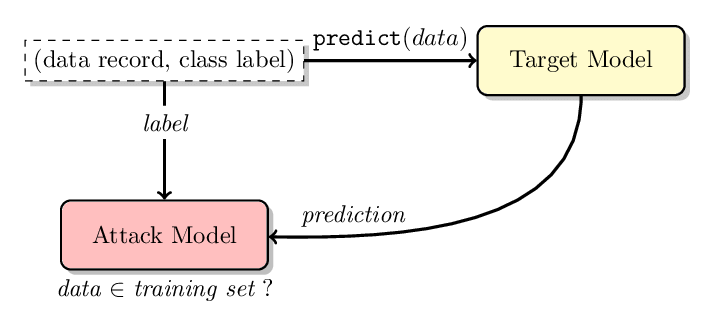
\includegraphics[width=\linewidth]{Membership-inference-attack-in-the-black-box-setting-The-attacker-queries-the-target.png}
		\caption{Black-box MIA workflow showing the shadow model pipeline \cite{shokri2017}. In a healthcare context, the target model is a clinical prediction API and the shadow models are trained on data from the same clinical distribution.}
		\label{fig:blackbox_mia}
	\end{figure}
	
	\subsubsection{Federated Learning Membership Inference}
	The federated setting changes the attack surface fundamentally. Figure~\ref{fig:federated_mia} illustrates the procedure. Rather than querying an API, the adversary observes gradient updates shared by other participants or submitted by victims. A malicious aggregating server can apply gradient inversion techniques to approximately reconstruct individual training samples from submitted updates, going beyond membership inference to data reconstruction. Even a co-participant who cannot invert gradients can still perform update analysis: the magnitude and direction of gradient changes correlate with the presence of specific training samples, enabling membership inference against other institutions' patient records without any API access whatsoever. This makes federated learning a qualitatively different threat model from centralized deployment, requiring defenses at the gradient level rather than the output level.
	
	\begin{figure}[H]
		\centering
		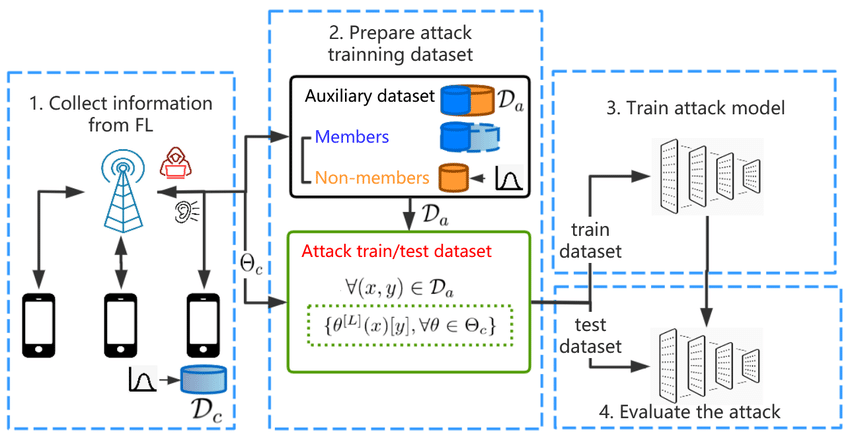
\includegraphics[width=\linewidth]{The-procedure-of-our-membership-inference-attack-on-federated-learning-TH-c-are-the-set.png}
		\caption{Federated learning MIA procedure \cite{nasr2019}. Unlike Figure~1, the adversary here operates at the gradient level, enabling membership inference without any API query access and across institutional trust boundaries.}
		\label{fig:federated_mia}
	\end{figure}
	
	\subsubsection{Differential Privacy: Mechanism and Trade-offs}
	Differential privacy provides a formal bound on the information any single training record contributes to model outputs. The guarantee is: for any two datasets $D$ and $D'$ differing in exactly one record, and any output set $S$, $\Pr[\mathcal{M}(D) \in S] \leq e^\epsilon \cdot \Pr[\mathcal{M}(D') \in S] + \delta$, where $\epsilon$ is the privacy budget and $\delta$ is a small failure probability. In DP-SGD, this is achieved by clipping per-sample gradients to a maximum $\ell_2$ norm $C$ and adding Gaussian noise $\mathcal{N}(0, \sigma^2 C^2)$ at each training step. Figure~\ref{fig:dp_ml} illustrates the mechanism.
	
	The privacy-utility trade-off is non-trivial in healthcare. Empirical results on clinical tabular datasets show that $\epsilon = 1$ (strong privacy) can reduce AUC by 5--15 percentage points; $\epsilon = 10$ typically costs 2--5 percentage points; and $\epsilon > 50$ provides marginal privacy benefit. For a high-stakes prediction task such as sepsis prediction or cancer screening, even a 2-point AUC reduction may be clinically meaningful. This trade-off must be explicitly evaluated during model design and reported to clinical stakeholders, not treated as a background engineering decision.
	
	\begin{figure}[H]
		\centering
		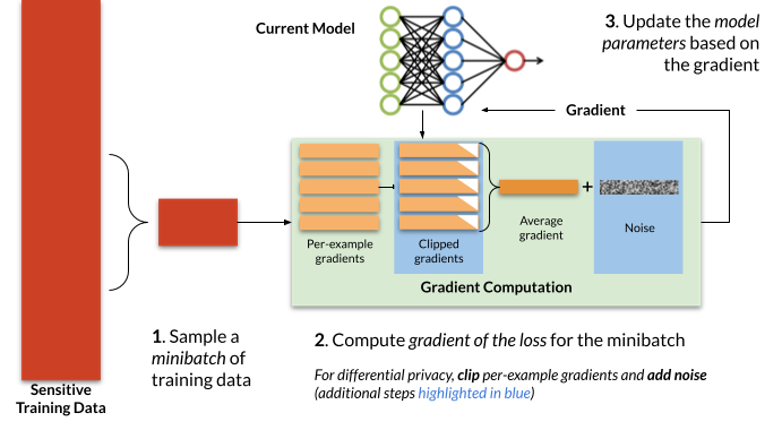
\includegraphics[width=0.92\linewidth]{DP-machine-learning-1.png}
		\caption{Differential privacy in the ML training loop \cite{img_dp}. Gradient clipping and noise addition bound each record's influence, directly limiting the signal an MIA attacker can exploit from model outputs.}
		\label{fig:dp_ml}
	\end{figure}
	
	\subsection{STRIDE Threat Model}
	Table~\ref{tab:stride} applies STRIDE to the medical AI system. Each category is mapped to a concrete MIA-relevant threat and primary mitigation.
	
	\begin{table}[H]
		\centering
		\caption{STRIDE threat model for medical AI membership inference}
		\label{tab:stride}
		\footnotesize
		\begin{tabularx}{\linewidth}{>{\raggedright\arraybackslash}p{1.55cm} >{\raggedright\arraybackslash}X >{\raggedright\arraybackslash}p{1.6cm}}
			\toprule
			Category & Threat in Healthcare AI Context & Primary Mitigation \\
			\midrule
			Spoofing & Stolen clinician credentials used to query inference API at scale & MFA, identity-aware API gateway \\
			Tampering & Adversarial manipulation of training inputs or federated updates & Input validation, anomaly detection \\
			Repudiation & No tamper-evident log of who queried the API and when & Immutable audit logging \\
			Info.\ Disclosure & Confidence scores leak training-set membership & Output truncation, DP, query budgets \\
			Denial of Service & High-volume probing disrupts service and funds shadow model & Rate limiting, per-principal caps \\
			Elevation of Privilege & Attacker gains model download access from registry & Registry RBAC, signed artifacts \\
			\bottomrule
		\end{tabularx}
	\end{table}
	
	The most critical category is Information Disclosure, since the model's own output is the primary attack surface. However, Elevation of Privilege is the highest-consequence escalation: if an adversary moves from API-level access to model weights, the attack shifts from black-box to white-box, dramatically amplifying membership leakage. Denial of Service is also directly attack-enabling: high-volume probing that disrupts the service may not be separable from shadow model data collection. The STRIDE analysis shows that effective MIA defense requires controls at all six threat categories simultaneously.
	
	\subsection{Formal Attack Tree}
	Figure~\ref{fig:attacktree} presents a formal attack tree decomposing the goal of ``Infer patient membership in a healthcare AI training cohort'' into sub-goals, AND/OR logic, and leaf-level attack steps. AND-nodes (double bar) require all children to succeed; OR-nodes (single bar) require at least one child. Each leaf is labeled with its attacker tier and a difficulty rating (L~=~Low, M~=~Medium, H~=~High), reflecting the practical barrier an adversary faces.
	
	\begin{figure*}[t]
		\centering
		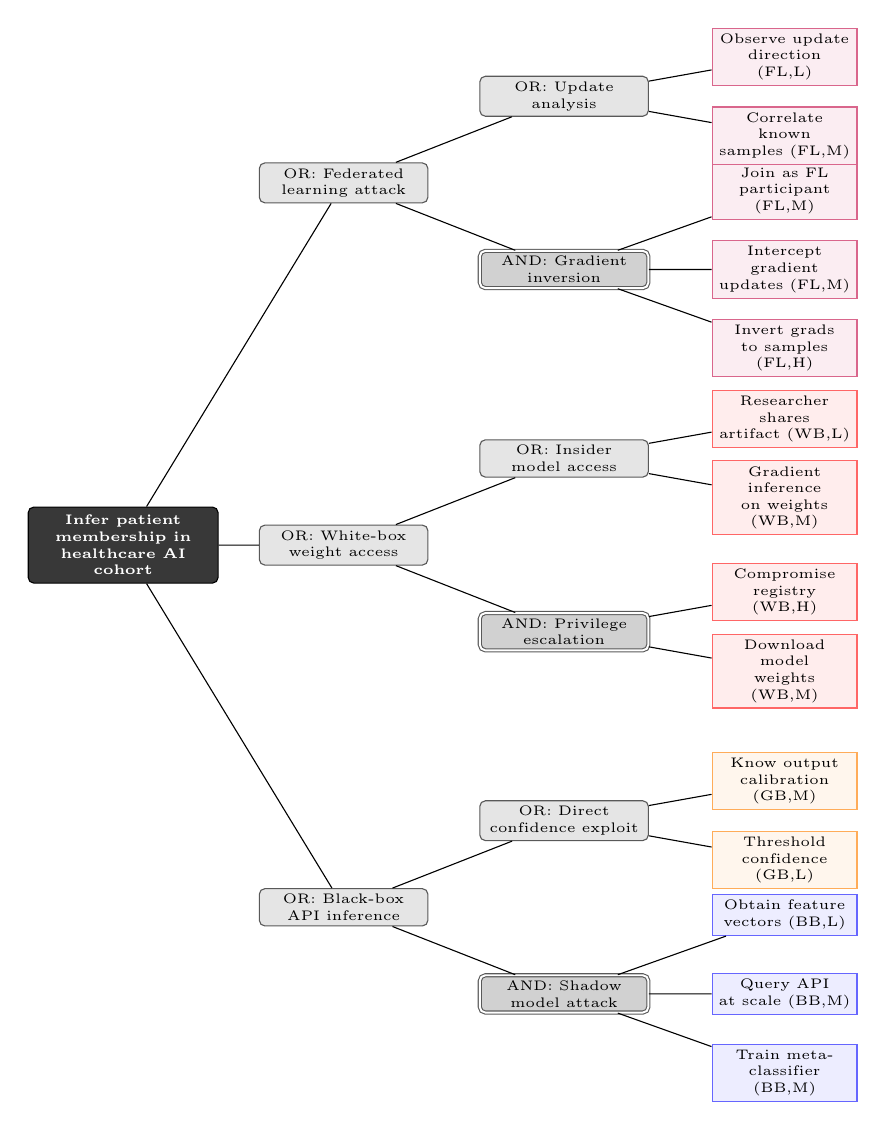
\begin{tikzpicture}[
			font=\tiny,
			every node/.style={align=center},
			grow=right,
			edge from parent/.style={draw,-},
			level distance=28mm,
			level 1/.style={sibling distance=46mm},
			level 2/.style={sibling distance=22mm},
			level 3/.style={sibling distance=10mm},
			goal/.style={rectangle, rounded corners=2pt, draw=black, fill=black!78,
				text=white, font=\tiny\bfseries, inner sep=3pt, text width=22mm},
			ornode/.style={rectangle, rounded corners=2pt, draw=black!65, fill=black!10,
				inner sep=2pt, text width=20mm},
			andnode/.style={rectangle, rounded corners=2pt, draw=black!65, fill=black!18,
				double, double distance=0.7pt, inner sep=2pt, text width=20mm},
			bb/.style={rectangle, draw=blue!60,   fill=blue!7,   inner sep=2pt, text width=17mm},
			gb/.style={rectangle, draw=orange!65, fill=orange!7,  inner sep=2pt, text width=17mm},
			wb/.style={rectangle, draw=red!60,    fill=red!7,    inner sep=2pt, text width=17mm},
			fl/.style={rectangle, draw=purple!60, fill=purple!7, inner sep=2pt, text width=17mm},
			]
			
			\node[goal] {Infer patient\\membership in\\healthcare AI\\cohort}
			child {
				node[ornode] {OR: Black-box\\API inference}
				child {
					node[andnode] {AND: Shadow\\model attack}
					child { node[bb] {Train meta-\\classifier (BB,M)} }
					child { node[bb] {Query API\\at scale (BB,M)} }
					child { node[bb] {Obtain feature\\vectors (BB,L)} }
				}
				child {
					node[ornode] {OR: Direct\\confidence exploit}
					child { node[gb] {Threshold\\confidence (GB,L)} }
					child { node[gb] {Know output\\calibration (GB,M)} }
				}
			}
			child {
				node[ornode] {OR: White-box\\weight access}
				child {
					node[andnode] {AND: Privilege\\escalation}
					child { node[wb] {Download model\\weights (WB,M)} }
					child { node[wb] {Compromise\\registry (WB,H)} }
				}
				child {
					node[ornode] {OR: Insider\\model access}
					child { node[wb] {Gradient inference\\on weights (WB,M)} }
					child { node[wb] {Researcher shares\\artifact (WB,L)} }
				}
			}
			child {
				node[ornode] {OR: Federated\\learning attack}
				child {
					node[andnode] {AND: Gradient\\inversion}
					child { node[fl] {Invert grads\\to samples (FL,H)} }
					child { node[fl] {Intercept gradient\\updates (FL,M)} }
					child { node[fl] {Join as FL\\participant (FL,M)} }
				}
				child {
					node[ornode] {OR: Update\\analysis}
					child { node[fl] {Correlate known\\samples (FL,M)} }
					child { node[fl] {Observe update\\direction (FL,L)} }
				}
			};
			
		\end{tikzpicture}
		
		\vspace{4pt}
		\scriptsize
		\colorbox{blue!7}{\strut\,BB\,}=Black-box\quad
		\colorbox{orange!7}{\strut\,GB\,}=Gray-box\quad
		\colorbox{red!7}{\strut\,WB\,}=White-box\quad
		\colorbox{purple!7}{\strut\,FL\,}=Federated\quad
		Double border=AND-node.\quad
		L=Low,\ M=Medium,\ H=High difficulty.
		\caption{Formal attack tree for MIA against a healthcare AI system (horizontal layout, root at left). The root decomposes via OR into three primary paths: black-box API inference, white-box weight access, and federated gradient-level inference. AND-nodes (double border) require all children; OR-nodes require one. Black-box attacks are low-to-medium cost; white-box attacks require privilege escalation (H) or insider sharing (L); federated attacks bypass all API-level controls entirely.}
		\label{fig:attacktree}
	\end{figure*}
	
	\subsection{Secure Architecture Design}
	Figure~\ref{fig:arch} summarizes the layered defense architecture for a Zero Trust-compliant healthcare AI deployment.
	
	\begin{figure}[H]
		\centering
		\footnotesize
		\setlength{\tabcolsep}{3pt}
		\begin{tabular}{|p{7.5cm}|}
			\hline
			\textbf{Layer 6: Governance \& Audit}\\
			Tamper-evident logs, privacy auditing (ML Privacy Meter), DPIAs, incident response\\
			\hline
			\textbf{Layer 5: Output Controls}\\
			Top-1 class only where clinically sufficient; confidence rounding; per-principal query budgets\\
			\hline
			\textbf{Layer 4: API Gateway}\\
			Identity-aware proxy, MFA enforcement, rate limiting, anomaly detection for probing patterns\\
			\hline
			\textbf{Layer 3: Model Registry}\\
			RBAC/ABAC, cryptographic signing of artifacts, restricted export, HSM-backed key management\\
			\hline
			\textbf{Layer 2: Training Infrastructure}\\
			DP-SGD with calibrated $\epsilon$; federated: SecAgg + local DP + participant attestation\\
			\hline
			\textbf{Layer 1: Data Layer}\\
			Encryption at rest (AES-256); access controls; data minimization; PQ-safe key management\\
			\hline
		\end{tabular}
		\caption{Layered Zero Trust defense architecture for healthcare AI. Each layer targets a distinct part of the MIA attack surface: data-layer controls reduce raw exposure; training-layer DP limits leakage at the source; registry controls prevent white-box escalation; API and output controls raise the cost of black-box attacks; governance provides detection and accountability.}
		\label{fig:arch}
	\end{figure}
	
	Each layer targets a distinct adversary type. The training layer controls (DP-SGD, SecAgg) address the federated participant and white-box adversaries by limiting the information encoded in model weights and gradients. The output and API controls address the black-box and gray-box adversaries by restricting and budgeting the signal available through API queries. The registry and governance layers prevent escalation and provide the audit trail required for regulatory compliance.
	
	\section{Results and Discussion}
	\subsection{Real-World Attack Scenario}

Consider a hospital deploying an AI model trained on patients enrolled in an HIV treatment program. An attacker with access to the inference API submits patient data obtained from external sources such as insurance records or leaked medical summaries. By analyzing the model's output probabilities and applying a membership inference classifier, the attacker can estimate whether a specific individual was part of the training dataset.
This directly reveals the individual's likely HIV-positive status without exposing any raw medical records. The attack operates through black-box access and exploits confidence differences caused by overfitting. In practice, this can produce insurance discrimination, employment risk, and social stigma without triggering a traditional breach notification process.
	\subsection{Patient Privacy Risk Analysis}
	The key question is: what exactly is leaked when membership is successfully inferred, and what harms follow? The answer depends on the training cohort. Table~\ref{tab:leakage} maps cohort types to specific leaked facts and potential harms.
	
	\begin{table}[H]
		\centering
		\caption{Leakage-to-harm mapping for healthcare MIA by cohort type}
		\label{tab:leakage}
		\scriptsize
		\begin{tabularx}{\linewidth}{>{\raggedright\arraybackslash}p{1.7cm} >{\raggedright\arraybackslash}X >{\raggedright\arraybackslash}X}
			\toprule
			Cohort Type & Fact Revealed by Membership & Potential Harm \\
			\midrule
			HIV treatment registry & HIV-positive status & Insurance denial, employment discrimination, stigma \\
			Addiction recovery program & Substance use disorder & Employment, custody, housing consequences \\
			Rare disease study & Specific genetic diagnosis & Insurability, family implications \\
			Psychiatric records & Mental health treatment history & Employment, security clearance, relationships \\
			Oncology clinical trial & Cancer diagnosis or treatment & Insurance, employment, financial harm \\
			\bottomrule
		\end{tabularx}
	\end{table}
	
	This table makes clear that MIA harm is not generic: it maps directly to the specific clinical meaning of cohort membership. A binary membership answer --- yes or no --- is sufficient to trigger concrete legal, financial, and social harm for patients in these cohorts. Unlike a data breach, this harm can materialize silently, with no breach notification triggered and no audit trail unless tamper-evident API logging is in place.
	
	The connection to overfitting is practically important. Healthcare datasets are frequently small relative to task complexity: a model trained on 500 rare disease cases may have a training-test AUC gap of 10 points or more, which Yeom et al.\ \cite{yeom2018} show directly bounds MIA advantage. Organizations should treat large generalization gaps as privacy warnings.
	
Recent studies show that membership inference attacks can perform substantially above random guessing. Shokri et al.\ reported strong attack performance against machine learning models, and later work showed that leakage remains significant even in more modern settings \cite{shokri2017,carlini2022}. In healthcare environments, where datasets are often smaller and more specialized, even moderate attack success is operationally serious because each successful inference may reveal highly sensitive clinical information.
	
	\subsection{Risk Matrix and Deployment Scenario Comparison}
	Table~\ref{tab:risk} classifies risk across five deployment scenarios. Figure~\ref{fig:arch} shows which defense layers are most relevant in each.
	
	\begin{table}[H]
		\centering
		\caption{Risk matrix: MIA likelihood and impact by deployment scenario}
		\label{tab:risk}
		\scriptsize
		\begin{tabularx}{\linewidth}{>{\raggedright\arraybackslash}X >{\raggedright\arraybackslash}p{1.1cm} >{\raggedright\arraybackslash}p{1.1cm} >{\raggedright\arraybackslash}p{1.0cm}}
			\toprule
			Scenario & Access & Likelihood & Impact \\
			\midrule
			Public API with confidence scores & Black-box & High & High \\
			Internal hospital model, strong IAM & Restricted & Low--Med & High \\
			Partner-shared downloadable model & White-box & High & High \\
			Federated hospital consortium & FL part. & Med--High & High \\
			Synthetic data release pipeline & Mixed & Medium & Med--High \\
			\bottomrule
		\end{tabularx}
	\end{table}
	
	Impact is uniformly high because cohort sensitivity is a property of the training data, not the deployment mode. Likelihood varies, which guides defense prioritization: public APIs and shared model artifacts require the most immediate technical controls (output truncation, query budgets, registry RBAC), while internal deployments can rely more heavily on IAM but still require logging and anomaly detection. The federated scenario requires a qualitatively different defense stack --- SecAgg and local DP rather than API-level controls --- because the attack surface is at the gradient level, not the output level.
	
	\subsection{Defense-to-Threat Mapping}
	Table~\ref{tab:defenses} explicitly maps each defense to the adversary type it addresses and its primary trade-off in a clinical context.
	
	\begin{table}[H]
		\centering
		\caption{Defense-to-threat mapping with clinical deployment trade-offs}
		\label{tab:defenses}
		\scriptsize
		\begin{tabularx}{\linewidth}{>{\raggedright\arraybackslash}p{1.8cm} >{\raggedright\arraybackslash}p{1.5cm} >{\raggedright\arraybackslash}X}
			\toprule
			Defense & Addresses & Clinical Trade-off \\
			\midrule
			DP-SGD ($\epsilon{<}10$) & All (source) & Reduces model AUC 2--15 pts depending on $\epsilon$; must be evaluated per task \\
			Output truncation & Black-box, gray-box & Hides confidence; acceptable if binary decision is clinically sufficient \\
			Query rate limiting & Black-box & No clinical impact; blocks shadow model data collection \\
			Registry RBAC & White-box & No clinical impact; prevents artifact escalation \\
			SecAgg (FL) & FL participant & Moderate compute overhead; prevents gradient inversion by aggregator \\
			Local DP (FL) & FL participant & Same accuracy trade-off as centralized DP; applied per institution \\
			Tamper-evident logs & All (detection) & No user-facing impact; enables forensic investigation \\
			\bottomrule
		\end{tabularx}
	\end{table}
	
	This mapping reveals an important asymmetry: system-level controls (rate limiting, registry RBAC, logging) impose no clinical cost and should be deployed unconditionally. Model-level controls (DP) carry accuracy costs and require deliberate calibration. Output controls (confidence truncation) require a clinical workflow review to confirm that binary outputs are sufficient. The practical recommendation is to deploy all system-level controls first, then layer DP at the highest $\epsilon$ that meets the accuracy threshold, then truncate outputs where clinically feasible.
	
	\subsection{Privacy and Regulatory Compliance}
	
	\subsubsection{HIPAA}
	HIPAA's Privacy Rule requires appropriate administrative, physical, and technical safeguards for PHI \cite{hipaa}. The de-identification safe harbor under 45 CFR \S 164.514 permits disclosure of data from which 18 specified identifiers have been removed, or for which expert determination certifies negligible re-identification risk. MIAs expose a structural gap in this framework: a model trained on de-identified records still encodes cohort statistics that support membership inference, particularly when the cohort is small or clinically specialized. An adversary who successfully infers that a patient was in the training cohort of an HIV treatment model has effectively learned a health fact, even though no PHI was disclosed at any point in the pipeline. HIPAA's current safe harbor was not designed with model-level leakage in mind, and regulators have not yet issued formal guidance addressing this gap.
	
	\subsubsection{GDPR}
	GDPR classifies health information as special-category personal data under Article 9, requiring explicit legal basis and strong safeguards. Article 35 mandates a Data Protection Impact Assessment for high-risk processing; clinical AI training would typically qualify \cite{gdpr}. Article 17's right to erasure creates a specific technical obligation for healthcare AI: if a patient requests deletion, the organization must demonstrate that the model no longer encodes the patient's data. This requires either model retraining, differential privacy guarantees strong enough to bound the patient's contribution, or machine unlearning techniques. Machine unlearning is an active research area without mature production tools, making GDPR compliance for models trained on erasable data a technically open problem.
	
	\subsubsection{PIPEDA}
	PIPEDA Principle 7 requires safeguards appropriate to the sensitivity of the information \cite{pipeda}. For medical AI, this means that as MIA techniques mature, organizations face an ongoing obligation to update their technical defenses, not merely those that existed at deployment time. The emergence of gradient inversion attacks in federated settings, for example, constitutes a new risk that existing safeguards may not address. Canadian healthcare AI operators should treat MIA as a known and material privacy risk and document it explicitly in privacy impact assessments.
	\subsection{Feasibility and Trade-Off Analysis}

While defenses such as differential privacy, output truncation, and secure aggregation reduce membership inference risk, they also introduce practical trade-offs. Differential privacy can reduce model accuracy, which may negatively affect clinical decision-making in high-stakes settings such as sepsis prediction or cancer screening. Output truncation reduces the confidence information available to attackers, but it may also reduce interpretability for clinicians who rely on probability scores as part of decision support.

Scalability is also a concern. Deploying layered defenses across large hospital networks requires coordination between institutions, standardized technical controls, and consistent regulatory compliance practices. Federated learning defenses such as secure aggregation and local differential privacy also increase computational overhead and implementation complexity.

From a long-term sustainability perspective, the most realistic approach is not a single defense but a layered one. System-level controls such as rate limiting, RBAC, and tamper-evident logging are easier to sustain operationally, while privacy-preserving training methods require ongoing calibration as models, data volumes, and clinical requirements evolve.
	\section{Cryptographic Analysis and Quantum Risk}
	
	\subsection{Classical Vulnerabilities and the Harvest-Now-Decrypt-Later Threat}
	Healthcare AI deployments rely on TLS for transport security, RSA and ECDSA for code signing and certificate management, and AES for data-at-rest encryption. Shor's algorithm, running on a sufficiently large fault-tolerant quantum computer, breaks RSA key exchange and ECDSA signatures in polynomial time. The practical threat for healthcare is not merely future-state: adversaries may be recording encrypted TLS traffic and signed model artifacts today for decryption once quantum hardware matures. Given that patient records are retained for 10 to 30 years and that fault-tolerant quantum computers are projected to be feasible within 10 to 20 years, the threat window for healthcare data is non-trivial.
	
	Grover's algorithm reduces symmetric key search to $O(\sqrt{2^n})$ steps, halving effective key length. AES-128 falls to roughly 64 effective bits, which is below recommended security margins. AES-256 retains approximately 128 effective bits and is considered sufficient. Organizations using AES-128 for patient data at rest should prioritize migration to AES-256 as a near-term action independent of the broader post-quantum transition.
	
	\subsection{Post-Quantum Transition Planning}
	NIST finalized three post-quantum standards in 2024: ML-KEM (FIPS 203) \cite{fips203} for key encapsulation, ML-DSA (FIPS 204) \cite{fips204} for digital signatures, and SLH-DSA (FIPS 205) \cite{fips205} for stateless hash-based signatures. Table~\ref{tab:pqc} summarizes the migration mapping.
	
	\begin{table}[H]
		\centering
		\caption{Post-quantum cryptographic transition for healthcare AI systems}
		\label{tab:pqc}
		\footnotesize
		\begin{tabularx}{\linewidth}{>{\raggedright\arraybackslash}p{2.0cm} >{\raggedright\arraybackslash}X >{\raggedright\arraybackslash}X}
			\toprule
			Function & Classical & Post-Quantum Target \\
			\midrule
			Key exchange & RSA, ECDH & ML-KEM (FIPS 203); hybrid TLS during transition \\
			Digital signatures & RSA, ECDSA & ML-DSA (FIPS 204); SLH-DSA (FIPS 205) for long-lived certs \\
			Data at rest & AES-128/256 & AES-256 immediately; PQ-safe key wrapping \\
			Model artifact signing & ECDSA & ML-DSA for registry-stored model artifacts \\
			\bottomrule
		\end{tabularx}
	\end{table}
	
	The link between post-quantum transition and MIA is direct: model artifacts stored in a registry are both high-value targets for white-box MIA and potentially encrypted with classical keys vulnerable to future quantum decryption. A stolen encrypted model artifact that cannot be decrypted today may be decrypted in a decade, enabling white-box membership inference against a cohort that no longer has any technical recourse. Healthcare organizations should treat model artifacts as sensitive long-lived assets subject to the same quantum transition urgency as patient records.
	
	A practical migration roadmap for healthcare AI includes: (1) cryptographic inventory of all systems and TLS endpoints; (2) crypto-agile PKI redesign to enable algorithm substitution; (3) near-term AES-256 migration for data at rest; (4) hybrid ML-KEM/ECDH TLS deployment; (5) ML-DSA signing of new model artifacts; and (6) prioritized re-encryption of high-sensitivity archived data and legacy model artifacts.
	
	\section{Ethical and Governance Considerations}
	Beyond legal compliance, MIAs raise fundamental ethical questions about the terms on which patients contribute data to healthcare AI. Patients who consent to treatment-related data use may not anticipate that their data will train models queryable by external parties, or that those models could later expose their participation in sensitive clinical programs. This consent gap is not merely theoretical: standard IRB-approved research consent forms and HIPAA authorizations were drafted before model-level privacy attacks were a recognized risk, and they do not address inference-based leakage.
	
	The harm is structurally asymmetric. For the majority of patients in a large general-purpose model, MIA risk may be low. But for patients in small, highly sensitive cohorts --- HIV treatment, addiction recovery, psychiatric care, rare genetic disease --- the risk of targeted membership inference is materially higher, and the consequences of exposure are severe. Stigma, employment discrimination, insurance denial, and family harm can follow from a single binary membership inference, entirely without a formal data breach or notification.
	
	Governance responses should include: explicit disclosure in research consent and HIPAA authorization forms that model training may occur; independent privacy auditing of deployed models using tools such as ML Privacy Meter prior to and after deployment; patient-accessible mechanisms to request model influence removal; institutional review of model-sharing and publication decisions that could convert internal black-box risk into external white-box risk; and data minimization applied to model outputs, not merely data collection. The principle of data minimization, central to GDPR Article 5 and PIPEDA Principle 4.4, requires that model outputs be limited to what is operationally necessary: if a clinical workflow requires only a binary prediction, exposing full probability vectors increases privacy risk without adding clinical value.
	
	\section{Conclusion and Future Work}
	Membership inference attacks represent a serious and underaddressed privacy threat in AI-based medical systems. The core insight of this paper is that MIA risk is not merely a model privacy problem: it is a combined failure of model design, system architecture, governance, and regulatory frameworks. A model that overfits to a small clinical cohort, is deployed behind a public API that returns full confidence vectors, is stored in a model registry accessible to consortium partners, and is encrypted with classical cryptographic keys is vulnerable at every layer simultaneously. Effective defense requires closing all of these gaps together.
	
	The practical priorities that emerge from this analysis are ordered by cost and urgency. System-level controls --- query rate limiting, registry RBAC, tamper-evident logging --- impose no clinical cost and should be deployed immediately in any healthcare AI system. DP-SGD should be applied at the highest $\epsilon$ consistent with clinical accuracy requirements, with the privacy-utility trade-off documented and reviewed by clinical stakeholders. Output truncation should be applied wherever binary outputs are clinically sufficient. Federated deployments require SecAgg and local DP as prerequisites, not optional add-ons. Post-quantum migration of TLS, model artifact signing, and data-at-rest key management should begin now, prioritizing assets with the longest expected retention periods.
	
	The convergence of federated learning adoption in healthcare with maturing gradient-inversion attacks is the most urgent emerging challenge. As more hospital consortia adopt federated training, the attack surface for membership inference expands to the gradient level across institutional trust boundaries, and the defenses required are qualitatively different from those sufficient for centralized deployment. Future work should address: standardized leakage auditing frameworks for clinical AI; stronger and more efficient federated defenses; machine unlearning methods capable of supporting GDPR Article 17 compliance at production scale; operational quantum-safe migration guidance for healthcare IT; and regulatory updates to HIPAA de-identification standards that account for model-level privacy risk.
	
	\section*{Appendix: Group Contribution Statements}
	\textbf{Member 1 (Mayankjot Singh):} Led threat modeling using STRIDE, defined the adversary model tiers, designed the layered architecture diagram, and developed the asset classification table. Validated STRIDE mappings against the reference system model and cross-checked adversary tier definitions against the academic literature. Key challenge: operationalizing the distinction between gray-box and white-box adversaries in realistic healthcare deployment contexts. AI tools were used to assist with drafting; all outputs were reviewed and validated against cited sources.
	
	\textbf{Member 2 (Ana Torres Landa Zarate):} Led the privacy law analysis covering HIPAA, GDPR, and PIPEDA, and contributed to the ethical and governance discussion. Analyzed the structural gap between HIPAA's de-identification safe harbor and model-level membership leakage, and synthesized regulatory obligations across three jurisdictions. Key lesson: de-identification is insufficient as a standalone privacy measure for AI-trained systems. AI tools were used for initial structuring; all regulatory analysis was verified against primary regulatory documents.
	
	\textbf{Member 3 (Ryll Santillan):} Led the attack mechanism analysis and differential privacy section, including the DP-SGD mathematical formulation and the privacy-utility trade-off discussion. Synthesized NIST PQC standards into the transition table and mapped post-quantum risk to model artifact sensitivity. Key challenge: translating theoretical DP guarantees into practical clinical deployment guidance. AI tools were used to assist with technical explanation drafts; outputs were refined against NIST publications and primary MIA papers.
	
	\textbf{Member 4 (Eric Ross):} Led the secure architecture section, federated learning defense analysis, and defense-to-threat mapping table. Researched SecAgg protocol mechanics, Zero Trust architecture controls for model inference APIs, and the interplay between rate limiting, output truncation, and registry controls as a combined black-box defense. Key lesson: system-level controls and model-level DP are complementary, not substitutes, and must be deployed together. AI tools were used for initial outlining; all architectural recommendations were validated against NIST SP 800-207 and primary sources.
	
	\textbf{Member 5 (Maaz Shahzad):} Led the results and discussion section including the leakage-to-harm mapping table, risk matrix, and deployment scenario comparison. Researched the practical implications of MIA risk for vulnerable patient populations, the asymmetric harm structure, and the limits of existing consent frameworks. Key challenge: articulating non-technical harm mechanisms with sufficient precision for a technically rigorous paper. AI tools were used for drafting support; all ethical and governance claims were grounded in regulatory frameworks and academic sources.
	
	\textbf{AI Tool Use Statement:} AI tools were used to assist with outlining, drafting, and refining technical explanations across all sections. All outputs were reviewed, edited, and validated against scholarly papers, NIST publications, and regulatory sources before inclusion. No AI-generated content was included without member review and validation of the underlying claims.
	
	\begin{thebibliography}{99}
		
		\bibitem{shokri2017}
		R. Shokri, M. Stronati, C. Song, and V. Shmatikov, ``Membership inference attacks against machine learning models,'' in \textit{Proc. IEEE Symp. Security Privacy}, 2017, pp. 3--18.
		
		\bibitem{yeom2018}
		S. Yeom, I. Giacomelli, M. Fredrikson, and S. Jha, ``Privacy risk in machine learning: Analyzing the connection to overfitting,'' in \textit{Proc. IEEE Comput. Secur. Found. Symp.}, 2018, pp. 268--282.
		
		\bibitem{nasr2019}
		M. Nasr, R. Shokri, and A. Houmansadr, ``Comprehensive privacy analysis of deep learning: Passive and active white-box inference attacks against centralized and federated learning,'' in \textit{Proc. IEEE Symp. Security Privacy}, 2019, pp. 739--753.
		
		\bibitem{nistzt}
		NIST, ``SP 800-207: Zero Trust Architecture,'' 2020.
		
		\bibitem{fips203}
		NIST, ``FIPS 203: Module-Lattice-Based Key-Encapsulation Mechanism Standard,'' 2024.
		
		\bibitem{fips204}
		NIST, ``FIPS 204: Module-Lattice-Based Digital Signature Standard,'' 2024.
		
		\bibitem{fips205}
		NIST, ``FIPS 205: Stateless Hash-Based Digital Signature Standard,'' 2024.
		
		\bibitem{hipaa}
		U.S. Department of Health and Human Services, ``Summary of the HIPAA Privacy Rule,'' 2025.
		
		\bibitem{gdpr}
		European Union, ``Regulation (EU) 2016/679: General Data Protection Regulation,'' 2016.
		
		\bibitem{pipeda}
		Office of the Privacy Commissioner of Canada, ``Personal Information Protection and Electronic Documents Act (PIPEDA).''
		
		\bibitem{carlini2022}
		N. Carlini, S. Chien, M. Nasr, S. Song, A. Terzis, and F. Tram\`{e}r, ``Membership inference attacks from first principles,'' in \textit{Proc. IEEE Symp. Security Privacy}, 2022, pp. 1565--1581.
		
		\bibitem{jagannathan2009}
		G. Jagannathan, K. Pillaipakkamnatt, and R. N. Wright, ``A practical differentially private random decision tree classifier,'' in \textit{Proc. IEEE Int. Conf. Data Mining Workshops}, 2009, pp. 114--121.
		
		\bibitem{bonawitz2017}
		K. Bonawitz, V. Ivanov, B. Kreuter, A. Marcedone, H. B. McMahan, S. Patel, D. Ramage, A. Segal, and K. Seth, ``Practical secure aggregation for privacy-preserving machine learning,'' in \textit{Proc. ACM SIGSAC Conf. Comput. Commun. Security}, 2017, pp. 1175--1191.
		
		\bibitem{img_dp}
		NIST, ``Differential privacy in machine learning,'' image resource, 2021.
		
	\end{thebibliography}
	
\end{document}
